\documentclass{beamer}
\usetheme{}
\usecolortheme{dolphin}           
\useinnertheme{circles}
\setbeamertemplate{itemize items}[default]
\setbeamertemplate{enumerate items}[default]
\usepackage[T1]{fontenc}
\usepackage[utf8]{inputenc}
\usepackage{lmodern}
\usepackage{amsmath}
\usepackage{booktabs} 
\usepackage{graphicx}        
\usepackage{array}
\usepackage{color}
\makeatletter
\def\zapcolorreset{\let\reset@color\relax\ignorespaces}
\def\colorrows#1{\noalign{\aftergroup\zapcolorreset#1}\ignorespaces}
\makeatother
\setbeamertemplate{navigation symbols}{}
\setbeamertemplate{footline}[frame number]

%--------------------------------------
\title{Optimum currency areas}
\author{School of Economics, University College Dublin}
\date{Spring 2018}
\begin{document}

%--------------------------------------
\begin{frame}
 \titlepage
\end{frame}
%--------------------------------------

%--------------------------------------
\begin{frame}
  Benefits of common currency area
  \begin{enumerate}
    \item Lowering of transaction costs
    \item Price transparency
    \item Uncertainty reduction
    \item Improvements in trade
    \item Quality of monetary policy
  \end{enumerate}
\end{frame}
%--------------------------------------

%--------------------------------------
\begin{frame}
  \textbf{Lowering of transaction costs}\\
  Occurs for two reasons
  \begin{enumerate}
    \item Common currency means that there is no need to discuss currency of transaction
    \item Elimination of exchange rate
  \end{enumerate}
  (2) means that there is no loss in value. 
  \begin{itemize}
    \item Changing from currency to currency can lead to 50\% loss
  \end{itemize}
  \medskip
  Additionally, lowering of costs might increase competition  
\end{frame}
%--------------------------------------

%--------------------------------------
\begin{frame}
  \textbf{Price transparency}\\
  Common currency means that prices are directly comparable across regions; again there are two effects
  \begin{enumerate}
    \item Increase in transparency might increase competition: good for consumers
    \item Can create trade opportunities: reducing border effect
    \begin{itemize}
      \item Border effect means that a national border is associated with a substantial reduction in trade
    \end{itemize}
  \end{enumerate}
\end{frame}
%--------------------------------------

%--------------------------------------
\begin{frame}
  Increased price transparency and competition will affect wage setting
    \begin{itemize}
    \item Note that countries compete with each other through exports
    \item Can become more competitive by adjusting wages   
    \item This is a long and painful process though
  \end{itemize}  
\end{frame}
%--------------------------------------

%--------------------------------------
\begin{frame}
  \textbf{Uncertainty reduction} stems from the elimination of the exchange rate
  \begin{itemize}
    \item Beneficial to foreign direct investment (FDI)
    \item FDI might be reduced due to long-term losses as a result of exchange rate fluctuations
  \end{itemize}
\end{frame}
%--------------------------------------

%--------------------------------------
\begin{frame}
  \textbf{Trade improvements}
  \begin{enumerate}
    \item Reduction of border effect
    \item Easier and more secure payment; might again increase competition
    \item Reduction in non-tariff barriers; reducing monopoly power
  \end{enumerate}
\end{frame}
%--------------------------------------

%--------------------------------------
\begin{frame}
  \textbf{Quality of monetary policy:} Idea is that policy will converge to a higher quality level for sub-par countries
  \begin{itemize}
    \item Common central bank will do better job that national central bank with low-quality
    \item Depends of course on quality of common central bank
  \end{itemize}
  \medskip
  Does involve loss of autonomy in monetary policy
\end{frame}
%--------------------------------------

%--------------------------------------
\begin{frame}
  Costs associated with common currency area
  \begin{enumerate}
    \item Link between shocks and exchange rate
    \item Dealing with asymmetric shocks
    \item Dealing with symmetric shocks that have asymmetric effects
  \end{enumerate}
  \medskip
  Costs stem mainly from cross-country differences
\end{frame}
%--------------------------------------

%--------------------------------------
\begin{frame}
  \textbf{Shocks and exchange rate}\\
  Country experiencing a shock can't lower exchange rate
  \begin{itemize}
    \item There are also no short-term alternatives
  \end{itemize}
  This means that the economy will slow-down for a prolonged time  
  \begin{figure}
    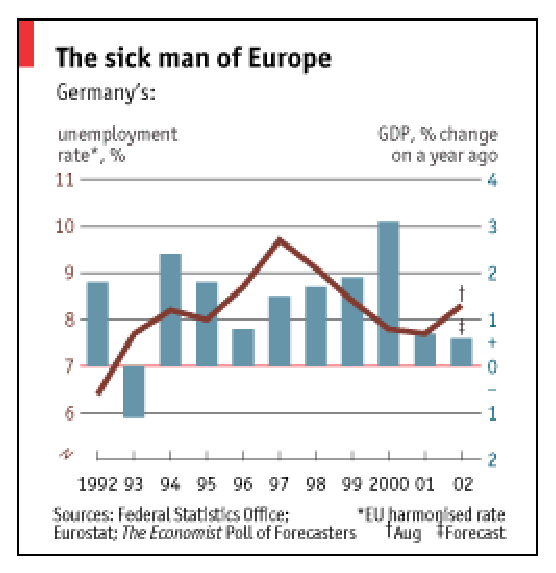
\includegraphics[scale=.4]{sick_man.eps}
  \end{figure}
\end{frame}
%--------------------------------------

%--------------------------------------
\begin{frame}
  \begin{figure}
    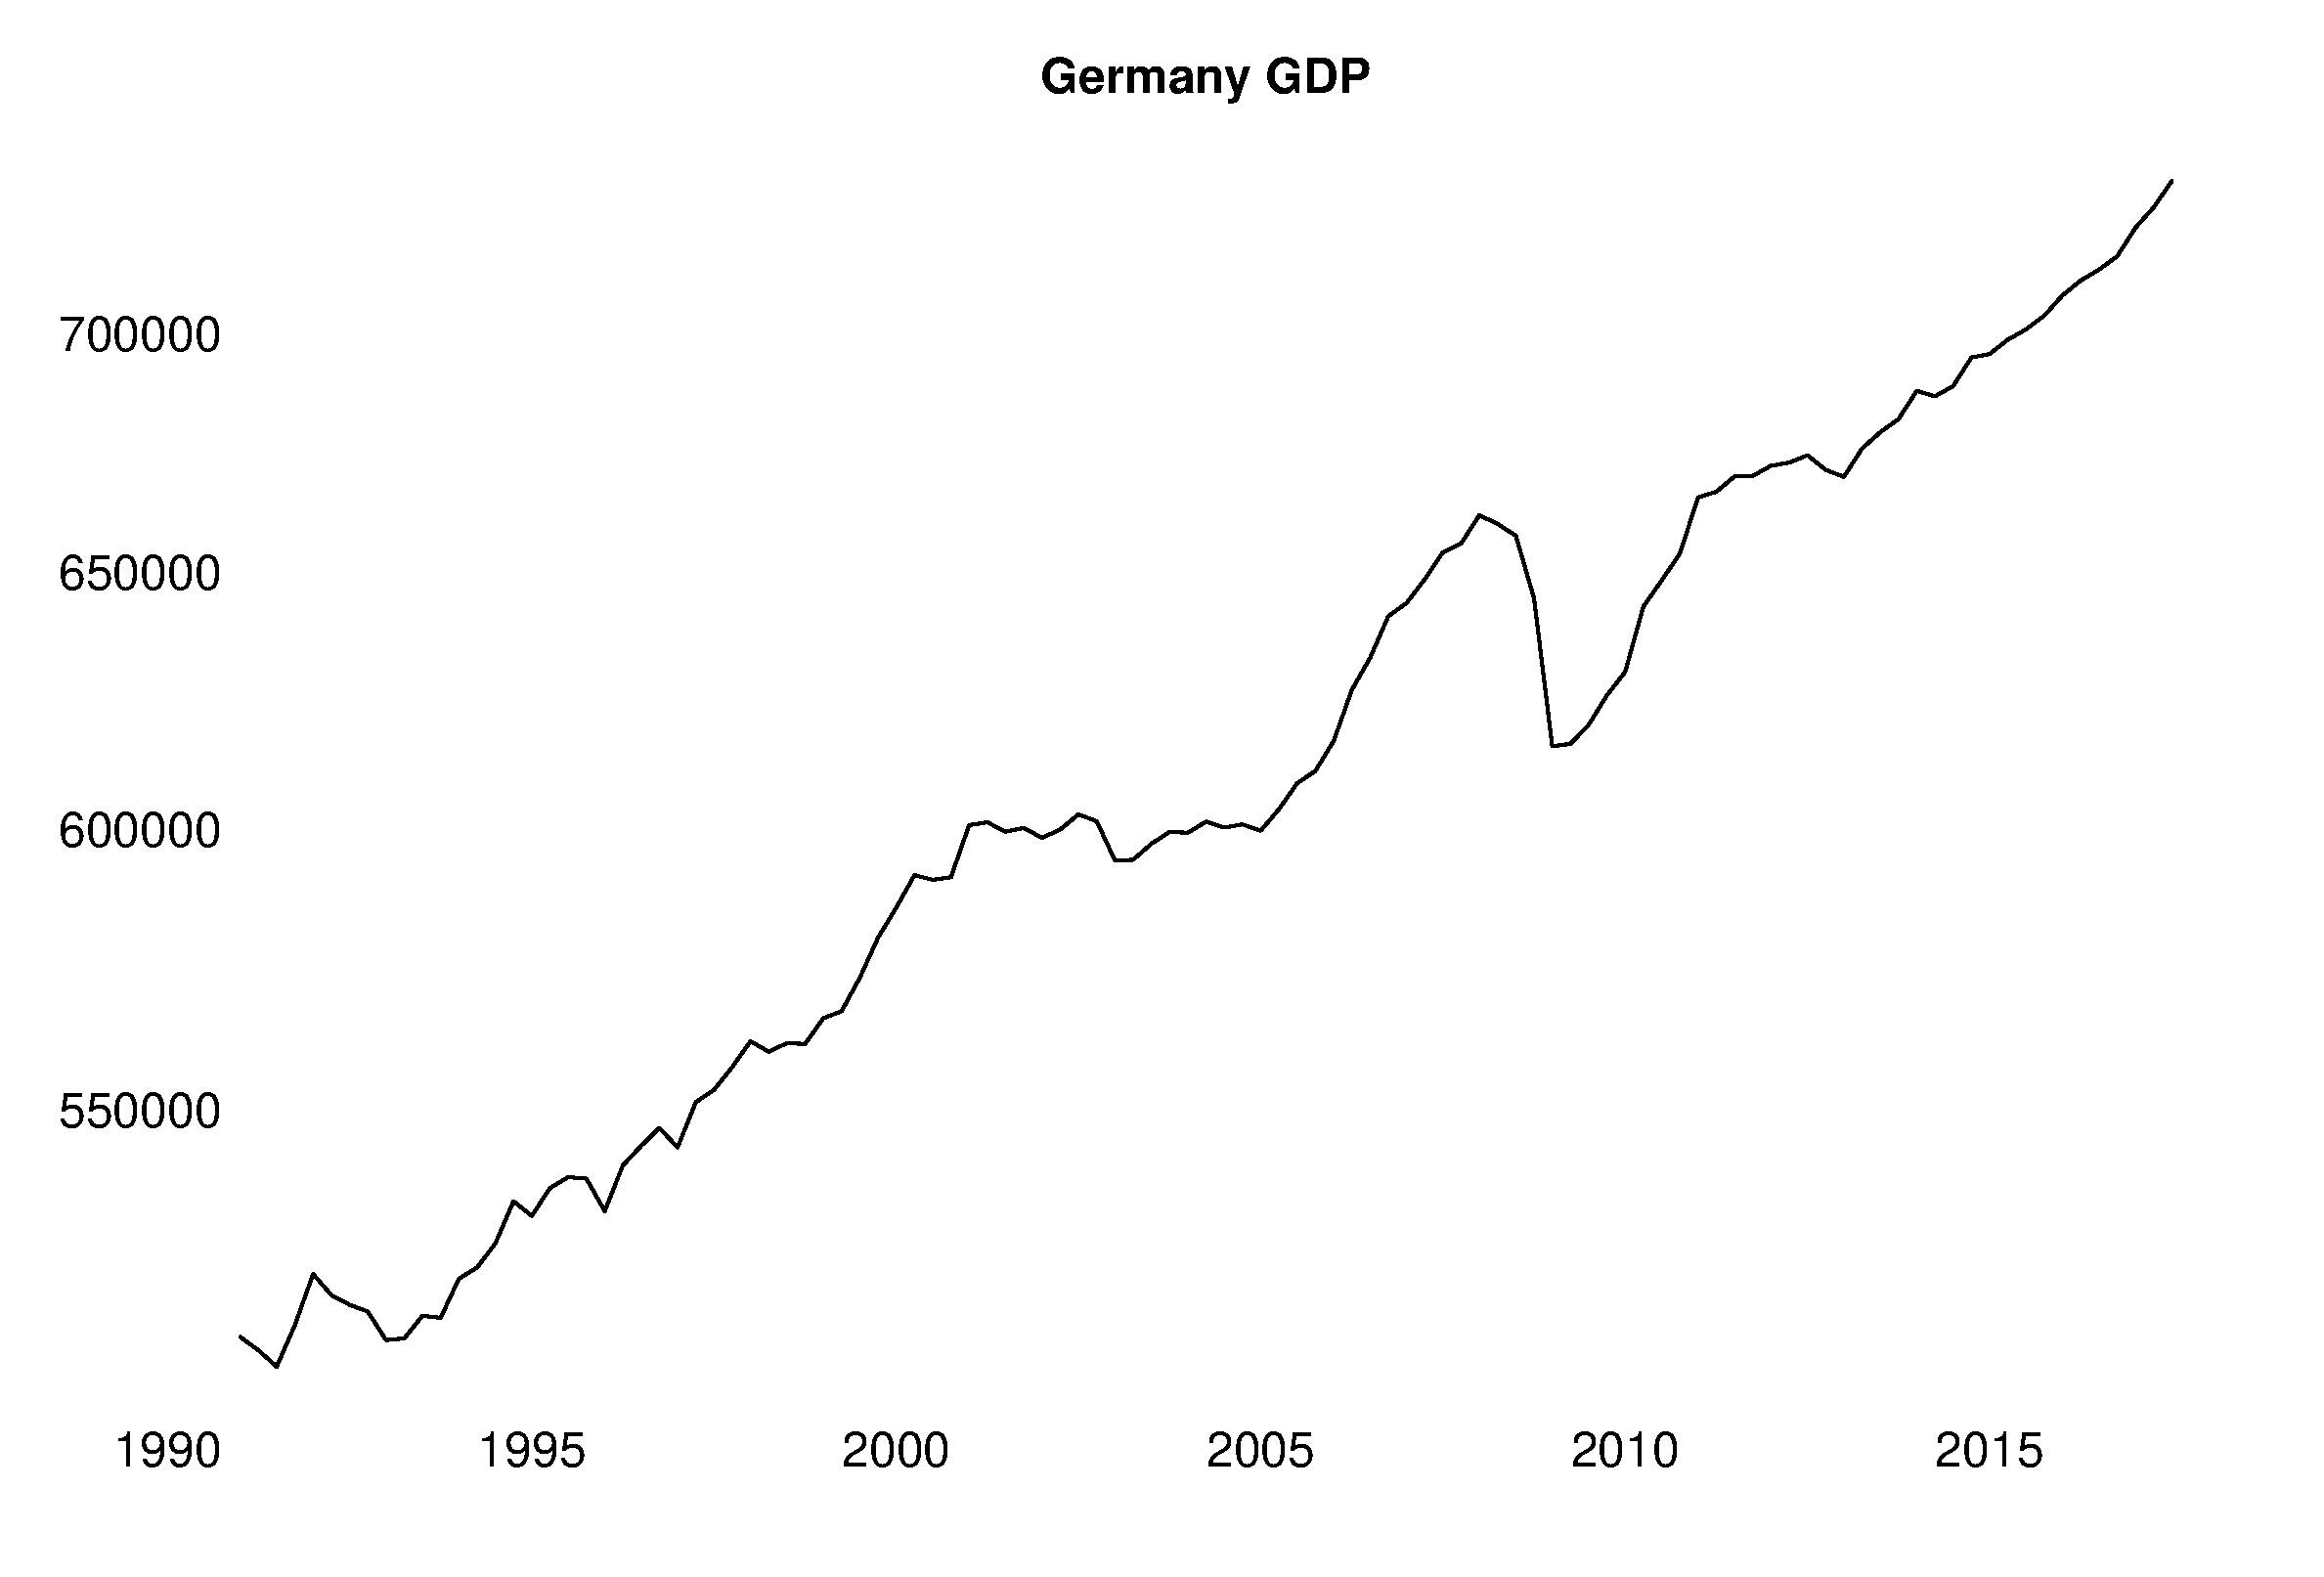
\includegraphics[scale=.3]{germany_gdp.eps}
  \end{figure}
\end{frame}
%--------------------------------------

%--------------------------------------
\begin{frame}
  \textbf{Asymmetric shocks}\\
  Countries will face different shocks when they have different characteristics
  \begin{itemize}
    \item e.g. Germany is not as earthquake-prone as Italy
  \end{itemize}
  \medskip
  What they do have in common in an OCA is the exchange rate
  \begin{itemize}
    \item When faced with an asymmetric shock, central bank has to make a decision
    \item This decision will likely have diverging effects: common exchange rate cannot insulate all countries
  \end{itemize}
\end{frame}
%--------------------------------------

%--------------------------------------
\begin{frame}
  \textbf{Symmetric shocks with asymmetric effects}: Countries experience same shock but react differently
  \begin{itemize}
    \item Result of socio-economic structure: labour regulations, external debt, etc.
  \end{itemize}
  \medskip
  Consider fall out of Brexit
  \begin{itemize}
    \item Ireland and Denmark exposed due to trade relations
    \item Poland and Portugal more insulated
  \end{itemize}
\end{frame}
%--------------------------------------

%--------------------------------------
\begin{frame}
  Common currency area criteria
  \begin{enumerate}
    \item Labour mobility
    \item Production diversification
    \item Openness
    \item Fiscal transfers
    \item Homogeneous preferences
    \item Cross-national solidarity
  \end{enumerate}
  \medskip
  Note that there are three economic and three political criteria
\end{frame}
%--------------------------------------

%--------------------------------------
\begin{frame}
  \textbf{Labour mobility:} 
  \begin{quote}
    In an OCA the people should be able to move easily between regions
  \end{quote}
  \medskip
  This in order to deal with shocks
  \begin{itemize}
    \item When factors of production can move freely shocks can be mitigated more easily
  \end{itemize}
  \medskip
  Various barriers to migration exist of course
  \begin{itemize}
    \item Cultural factors such as language
    \item Skill of the migrant worker
  \end{itemize}
\end{frame}
%--------------------------------------

%--------------------------------------
\begin{frame}
  \textbf{Production diversification}
  \begin{quote}
    Having a similar production structure and widely diversified production and exports is beneficial for a OCA
  \end{quote}
   Recall that asymmetric shocks are a large problem for currency areas. The question is, how often do these shocks occur?
  \begin{itemize}    
    \item If rare: costs will be episodic; profits accrue very day
  \end{itemize}
  \medskip
  Specialised economies will be more severely affects by shocks
  \begin{itemize}
    \item $Pr$(Asymmetric shock) reduced if countries produce similar goods in diversified economy
    \item Not clear how diversified economies should be
  \end{itemize}
\end{frame}
%--------------------------------------

%--------------------------------------
\begin{frame}
  \textbf{Openness} 
  \begin{quote}
    When countries are open to trade and trade heavily with each other, they could form an OCA
  \end{quote}
  \medskip
  In an OCA no distinction between domestic and foreign good
  \begin{itemize}
    \item Competition will equalise price of most goods when they are expressed in the same currency
    \item Changes in the exchange rate might affect competitiveness through exports; firms might want to focus on exports at certain price levels as it is more profitable.
  \end{itemize}
\end{frame}
%--------------------------------------

%--------------------------------------
\begin{frame}
 
\end{frame}
%--------------------------------------


%--------------------------------------
\begin{frame}
  \textbf{Fiscal transfers} 
  \begin{quote}
    When countries agree to compensate each other for adverse shocks, they form an OCA
  \end{quote}
  \medskip
  Note that there is a moral hazard issue here
  \begin{itemize}
    \item Countries might be expecting transfers to happen; might be slacking
    \item e.g. no diversified economy; heavy import dependence; rigid labour markets
  \end{itemize}
  \medskip
  Free-riding behaviour has been an important discourse during eurocrisis
  \begin{itemize}
    \item North vs. South
  \end{itemize}
\end{frame}
%--------------------------------------

%--------------------------------------
\begin{frame}
  \textbf{Homogeneous preferences}
  \begin{quote}
    Currency union member countries must reach consensus on the best way to deal with shocks
  \end{quote}
    \medskip
  \textbf{Solidarity vs. nationalism:}\\
   Common monetary policy might give rise to conflicts of national interests
  \begin{itemize}
    \item OCA member needs to accept the costs in the name of a common destiny
    \item Acceptable when
    \begin{align*}
      Costs < \sum Benefits
    \end{align*}    
  \end{itemize}
  This criteria also implies that there should be a move to a political union some time in the future
\end{frame}
%--------------------------------------

%--------------------------------------
\begin{frame}

\end{frame}
%--------------------------------------


%--------------------------------------
\begin{frame}
  \textbf{Labour mobility} is required in order to deal with asymmetric shocks but there are obstacles
  \medskip
\begin{itemize}
  \item The cost of moving itself
  \item The risk of becoming unemployed in the destination country
  \item Prospects for the family
  \item Fiscal factors such as social benefits and taxation on earnings
\end{itemize}
\end{frame}
%--------------------------------------

%--------------------------------------
\begin{frame}
  In addition to economic considerations there are other factors influencing the decision to migrate
  \begin{itemize}
    \item Cultural differences
    \item Links with family and friends
    \item Commitment to origin country
  \end{itemize}
  \medskip
  Combination of factors means that migration will be limited
\end{frame}
%-------------------------------------


%--------------------------------------
\begin{frame} 
  Can compare European labour mobility with US
  \begin{itemize}
    \item Similar geographic size
    \item Same level of economic development
    \item Comparable within-area differences: Greece is Europe's Mississippi
  \end{itemize}
\end{frame}
%--------------------------------------

%--------------------------------------
\begin{frame}
  \begin{figure}
    
\includegraphics[scale=.7]{eu_labour.eps}
  \end{figure}
\end{frame}
%--------------------------------------

%--------------------------------------
\begin{frame}
  \begin{figure}
    
\includegraphics[scale=.7]{eu_labour2.eps}
  \end{figure}
\end{frame}
%--------------------------------------

%--------------------------------------
\begin{frame}
  \begin{figure}
    
\includegraphics[scale=.7]{eu_labour3.eps}
  \end{figure}
\end{frame}
%--------------------------------------

%--------------------------------------
\begin{frame}
  \begin{figure}
    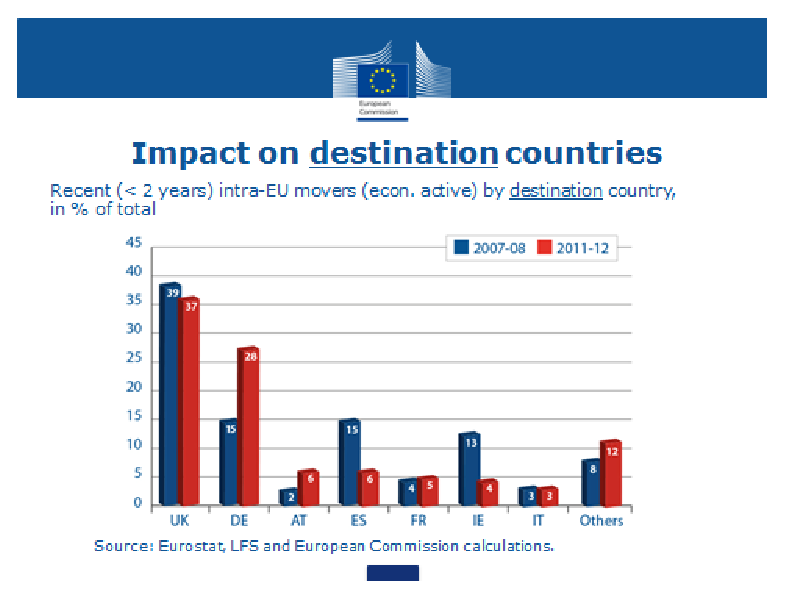
\includegraphics[scale=.7]{eu_labour4.eps}
  \end{figure}
\end{frame}
%--------------------------------------

%--------------------------------------
\begin{frame}
  Asymmetric shocks can have severe economic consequences leading to high levels of unemployment
  \begin{itemize}
    \item Specifically in the eurozone given low labour moblity levels
  \end{itemize}
  \medskip
  Therefore important that economies are 
  \begin{enumerate}
    \item Diversified
    \item Open to trade
  \end{enumerate}
  \medskip 
  Frequency of asymmetric shocks is lower among countries with
  \begin{itemize}
    \item Similar production patterns
    \item Diversified trade pattern
  \end{itemize}
\end{frame}
%--------------------------------------

%--------------------------------------
\begin{frame}
  \begin{figure}
    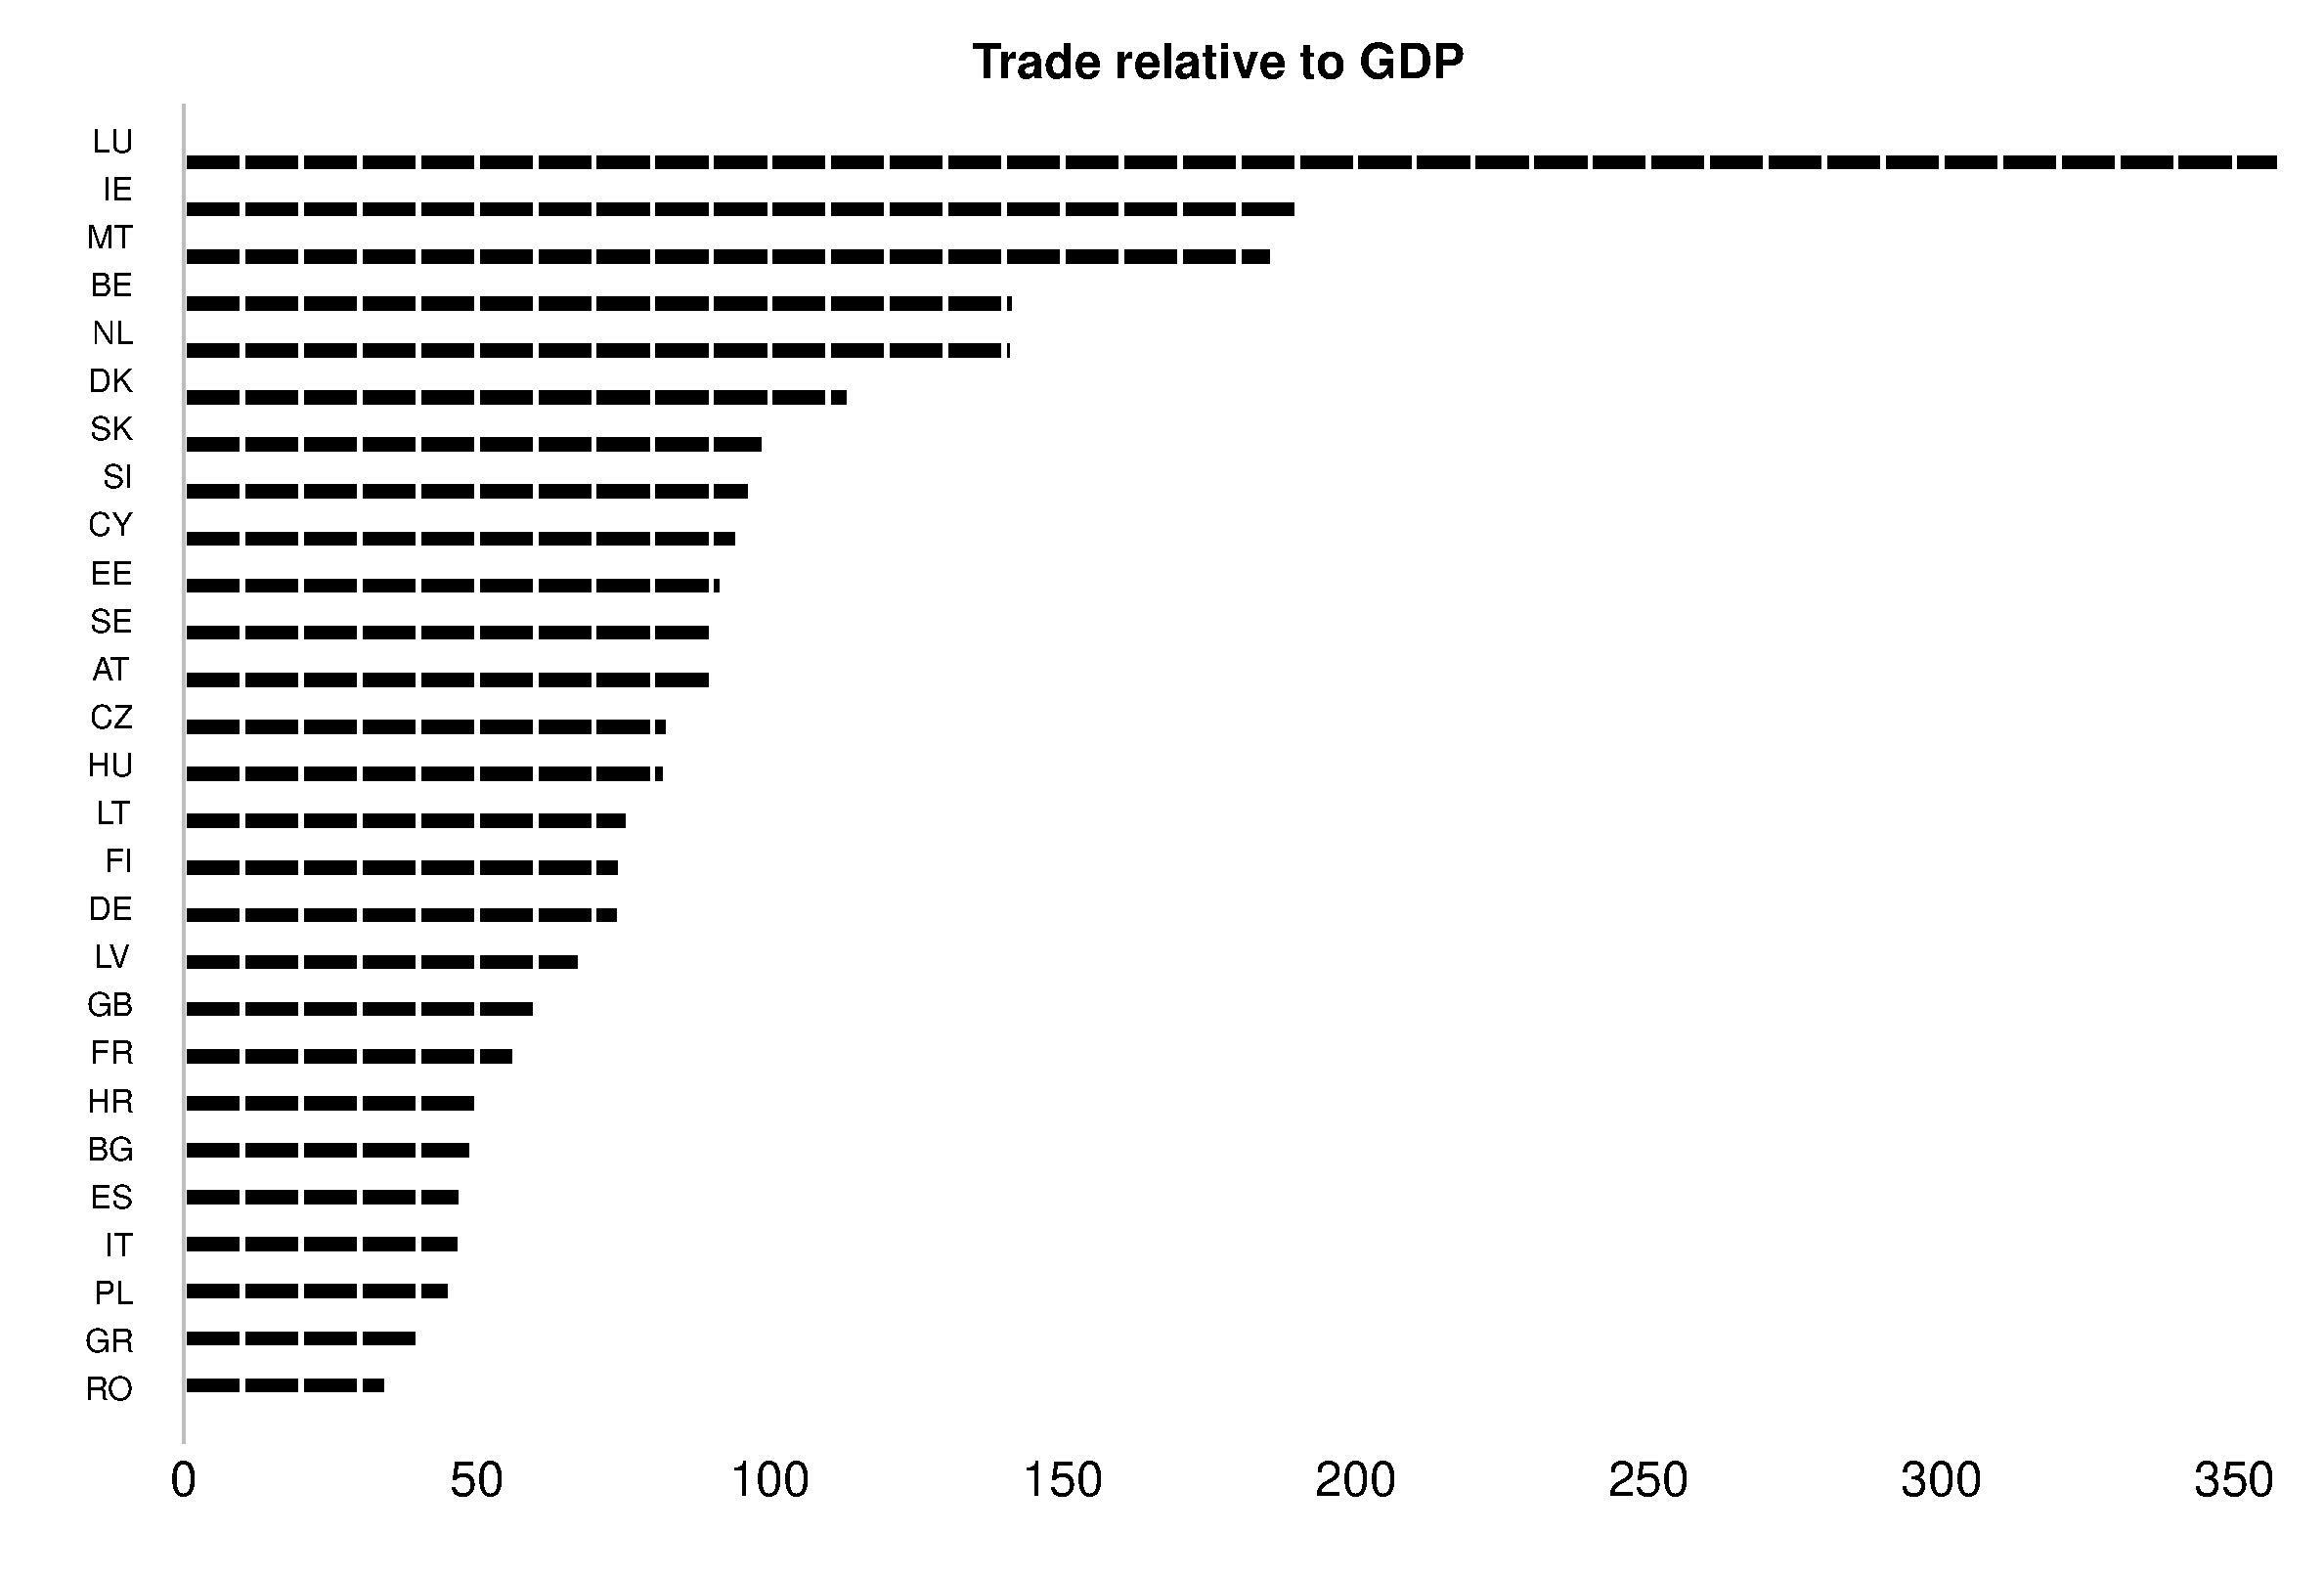
\includegraphics[scale=.3]{openness.eps}
  \end{figure}
\end{frame}
%--------------------------------------


%--------------------------------------
\begin{frame}
  \textbf{Homogeneous preferences} on monetary and fiscal policy is an import economic criteria. 
  \begin{itemize}
    \item Monetary policy is an important tool in dealing with shocks
  \end{itemize}
  \medskip
  To determine homogeneity in preference we should look at long term trends in
  \begin{enumerate}
    \item Inflation rate: for monetary policy
    \item Public debt levels: for fiscal policy
  \end{enumerate}
\end{frame}
%--------------------------------------


%--------------------------------------
\begin{frame}
  \begin{figure}
    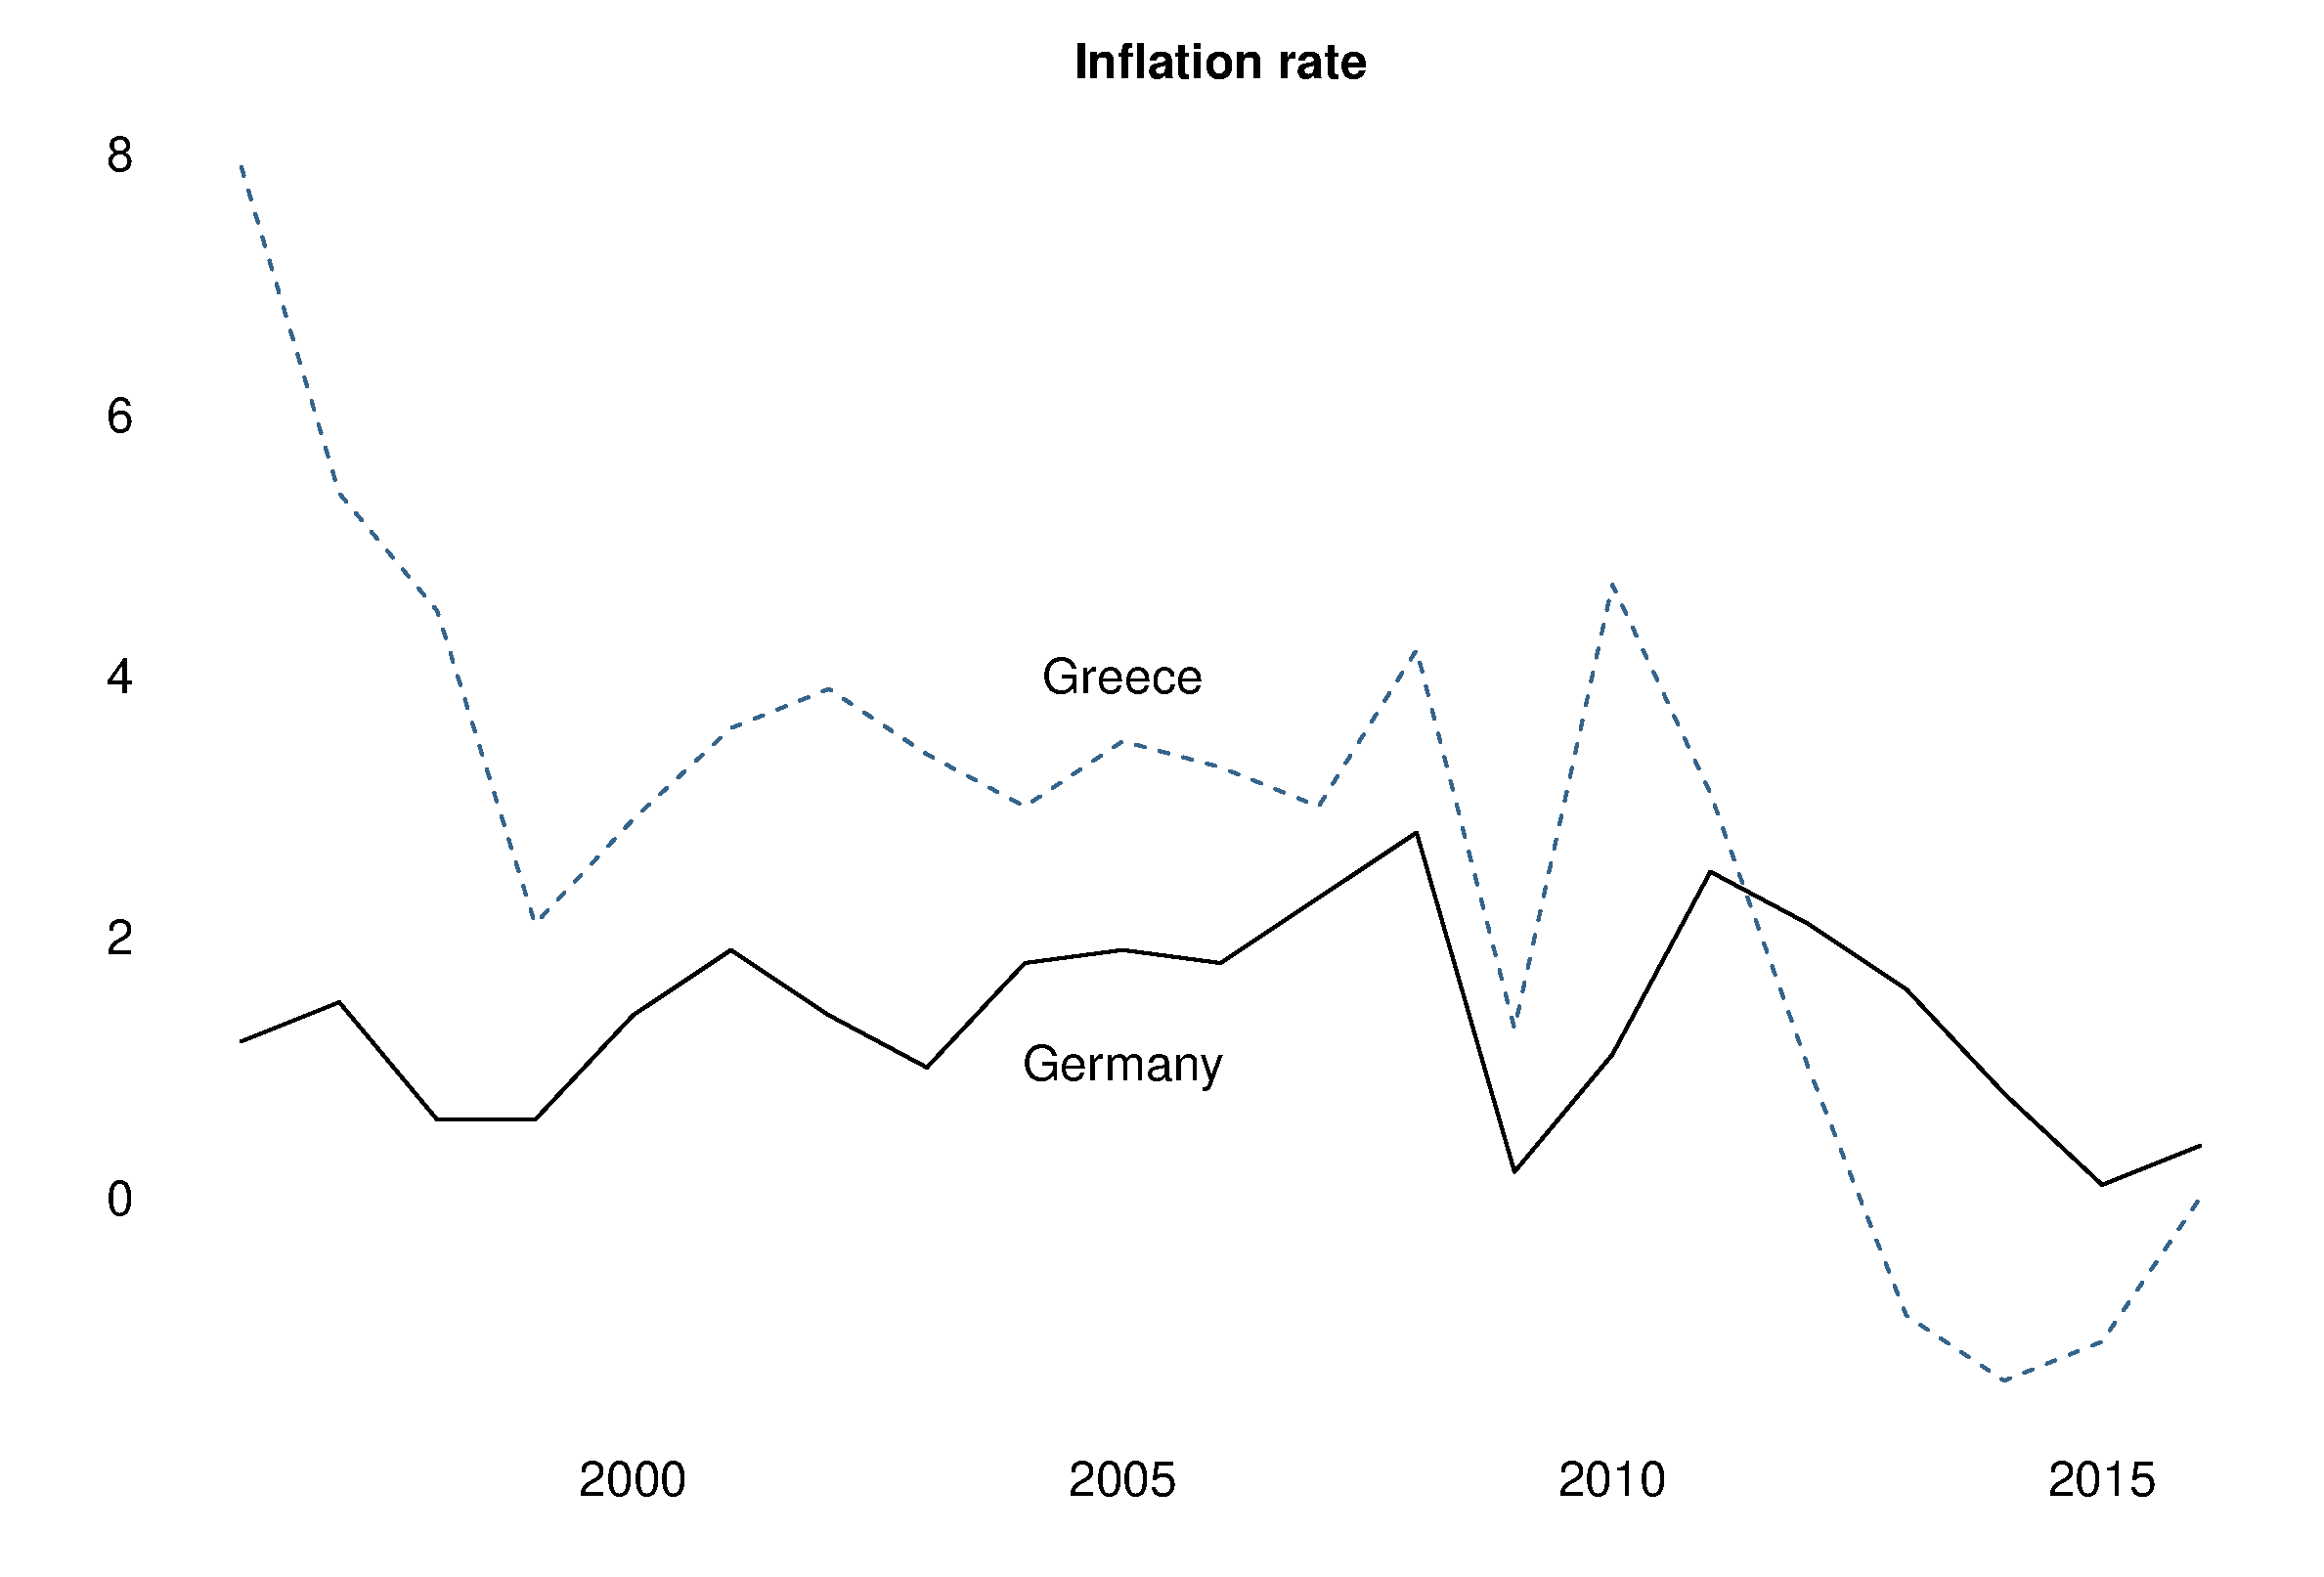
\includegraphics[scale=.3]{inflation.eps}
  \end{figure}
\end{frame}
%--------------------------------------

%--------------------------------------
\begin{frame}
  \begin{figure}
    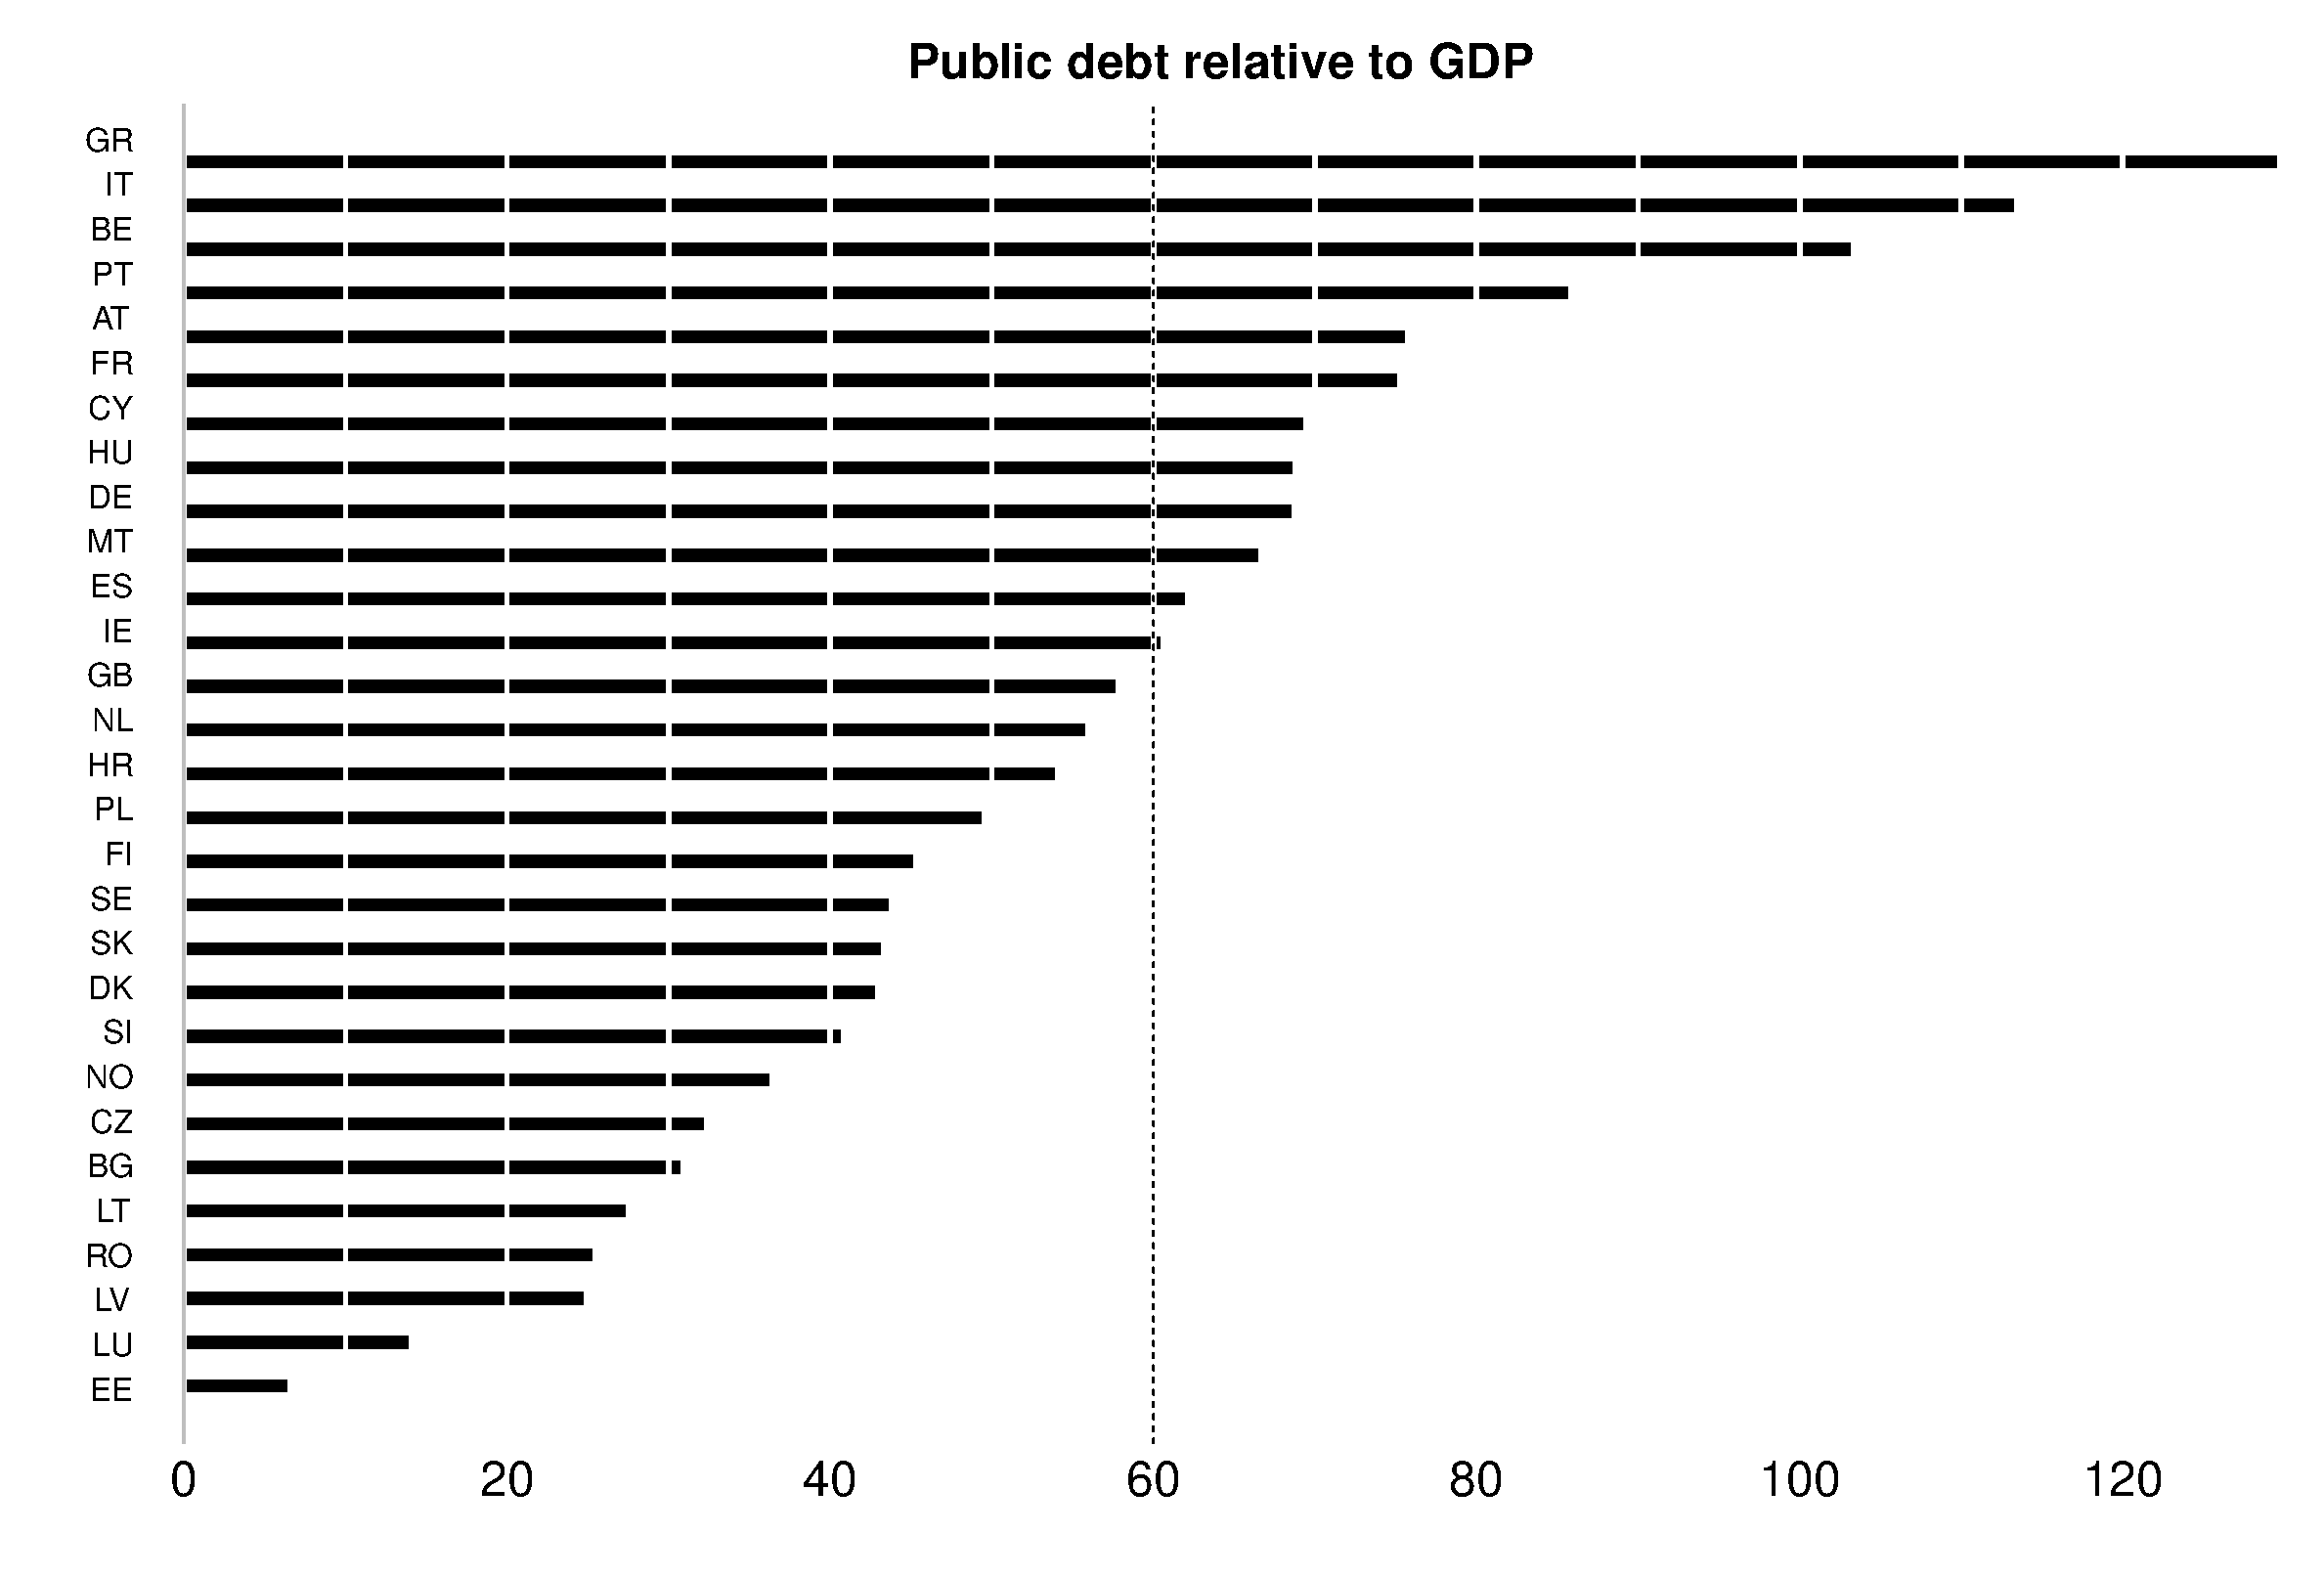
\includegraphics[scale=.3]{public_debt.eps}
  \end{figure}
\end{frame}
%--------------------------------------

%--------------------------------------
\begin{frame}
  What explains differences in macroeconomic policy across countries?
  \begin{itemize}
    \item Politician's incentives; shapes national institutions
    \item e.g. strong labour union movements; emphasis on public goods provision
  \end{itemize}
  \medskip
  To homogenise need to set up common institutions such as European Central Bank
  \begin{itemize}
    \item ECB determines monetary policy for eurozone
    \item Main objective: price stability
  \end{itemize}
\end{frame}
%--------------------------------------

%--------------------------------------
\begin{frame}
   In addition, all EU national budgets are subject to excessive debt procedure to curtail excessive public spending
  \begin{itemize}
    \item Operation under common institutions does not imply agreement on best course of action in dealing with shocks
  \end{itemize}
\end{frame}
%--------------------------------------


%--------------------------------------
\begin{frame}
  \textbf{Fiscal transfers:} One of the OCA criteria; let's check EU budget  
  \begin{enumerate}
    \item Structural fund and Cohesion policy (50\%)
    \item Common Agricultural Policy (43\%)
    \item Operating expenses (6\%)
  \end{enumerate}
  \medskip
  In general the budget of the European Union is very small at about only 1\% of the combined GDP of all EU member states. 
\end{frame}
%--------------------------------------

%--------------------------------------
\begin{frame}
  EU, or Eurozone, has no cyclical transfer system
  \begin{itemize}
    \item Structural fund/Cohesion policy transfers money to assist in stimulating economy in long-run
    \item EU regions with a GDP below 75\% of the EU average; regardless of shocks
    \item Transfers are for 7-year period and not cyclical
  \end{itemize}
\end{frame}
%--------------------------------------

%--------------------------------------
\begin{frame}
 Important first step towards fiscal transfers is the European Stability Mechanism (ESM)
  Some attempt at fiscal transfers following the Euro crisis; e.g. European Stability Mechanism
  \begin{itemize}
    \item Following the eurocrisis
    \item ESM member states can apply for ESM bailout when 
    \begin{enumerate}
      \item They are in serious financial difficulty
      \item Their banks need recapitalisation. 
    \end{enumerate}
  \end{itemize}       
\end{frame}
%--------------------------------------


%--------------------------------------
\begin{frame}
  \begin{figure}
    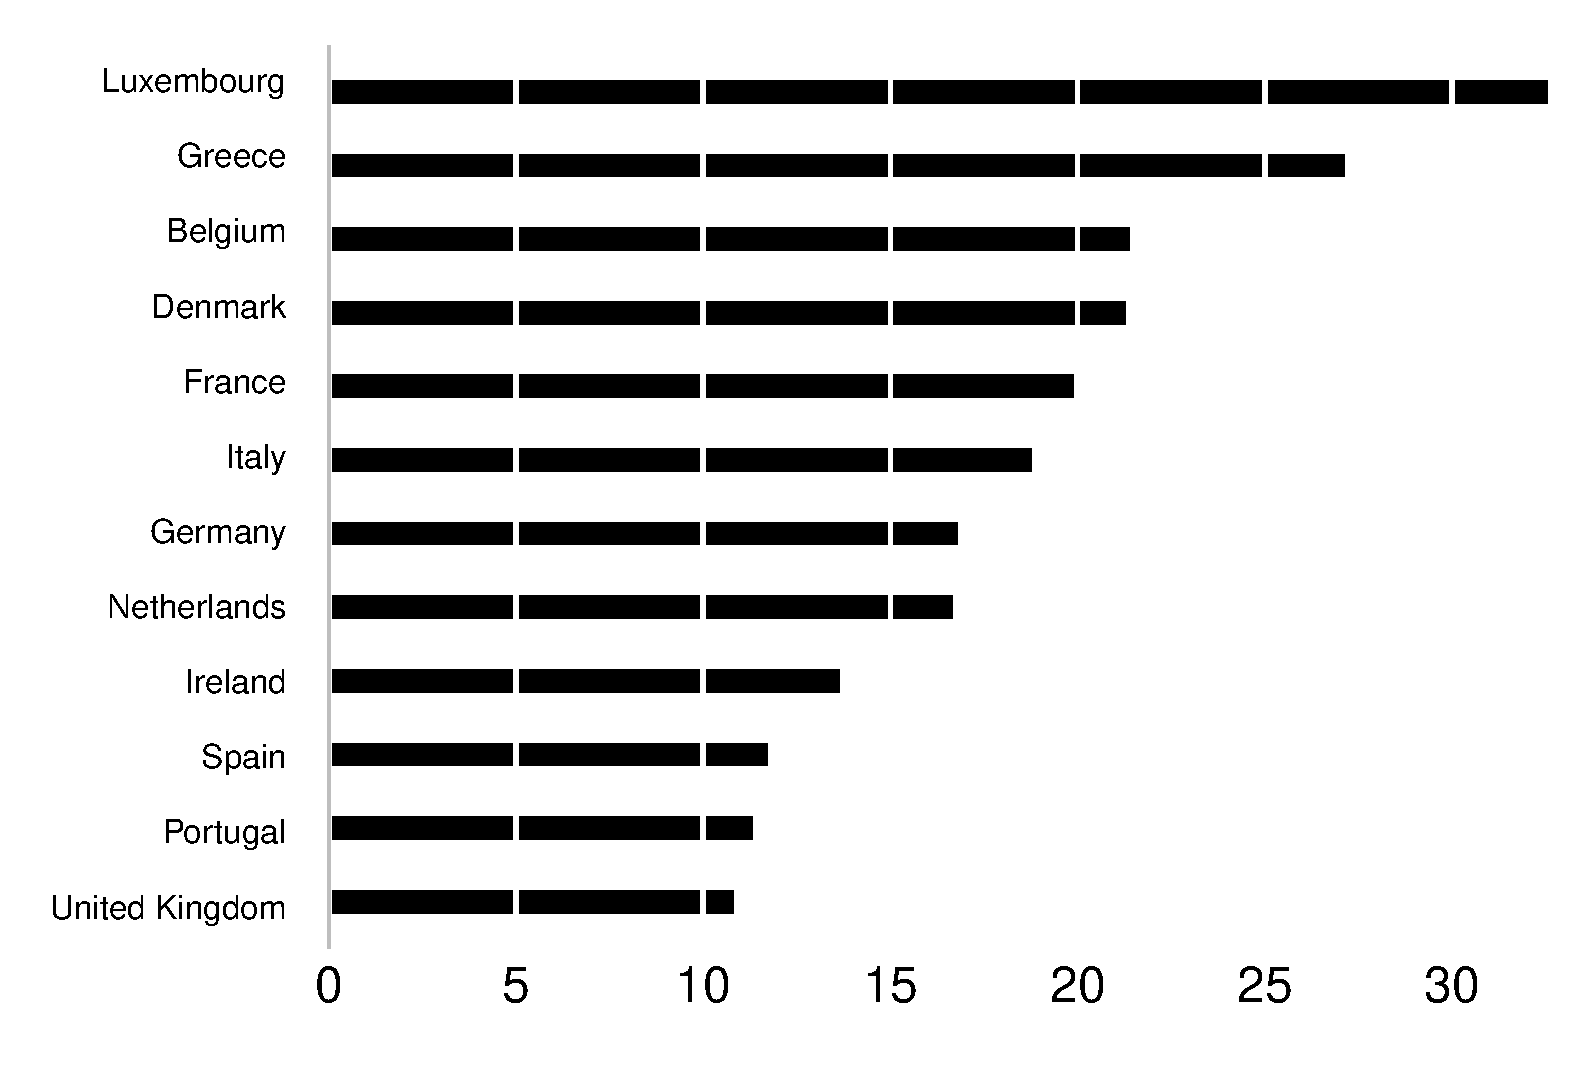
\includegraphics[scale=.4]{eurobarometer.eps}
  \end{figure}
\end{frame}
%--------------------------------------

%--------------------------------------
\begin{frame}
  European skepticism
  \begin{itemize}
    \item Rejection of EU constitution by French and Dutch voters
    \item Nativist movements across Europe (FRA,NLD, AUT, GER) following Great Recession
    \item Brexit
    \item Poland, Hungary
  \end{itemize}
  \medskip
  More enthusiastic supporters of European project can be found in
  \begin{itemize}
    \item Scotland, Catalonia
    \item Ukraine, Georgia
  \end{itemize}
\end{frame}
%--------------------------------------

%--------------------------------------
\begin{frame}
\begin{table}[!h] \centering \caption{Scorecard for the OCA criteria} \label{table:summary}
\scalebox{1}{\begin{tabular}{lc}
\\[-1.8ex]\hline 
\hline \\[-1.8ex] 
Criterion & Satisfied\\
\hline \\[-1.8ex]\\
Labour mobility & No\\
Trade openness  & Yes\\
Product diversification & Yes\\
Fiscal transfers & No\\
Homogeneous preferences & Partially\\
Commonality of destiny & Hard to tell\\
    \\[-1.8ex]\hline 
    \hline \\[-1.8ex]
\end{tabular} }  
\end{table}
\end{frame}
%--------------------------------------

%--------------------------------------
\begin{frame}
  \begin{enumerate}
  \item Euro project remains controversial
  \begin{itemize}
    \item Difficult to make a hard case for both supporters and opponents
    \item OCA criteria more guiding principle rather than iron law
    \item Decision to create a monetary union ultimately rests on political considerations
  \end{itemize}
  \medskip
  \item Given partial fulfillment of OCA criteria, going ahead will mean future costs
  \begin{itemize}
    \item Costs will mainly arise in the labour market and fiscal transfers
    \item Eurozone crisis showed that asymmetric shocks happen and can be painful
  \end{itemize}
\end{enumerate}
\end{frame}
%--------------------------------------

%--------------------------------------
\end{document}
